\section {Overall design}

The architecture of the entire system consists of different processes and modules which interact with each other. There are two distinct process types: persistent and non-persistent. The persistent processes will run for the entire uptime of the system whereas the lifetime of a non-persistent process is the duration of its given task. Figure x below shows the current system design.

\begin{figure}[h!]
	\centering
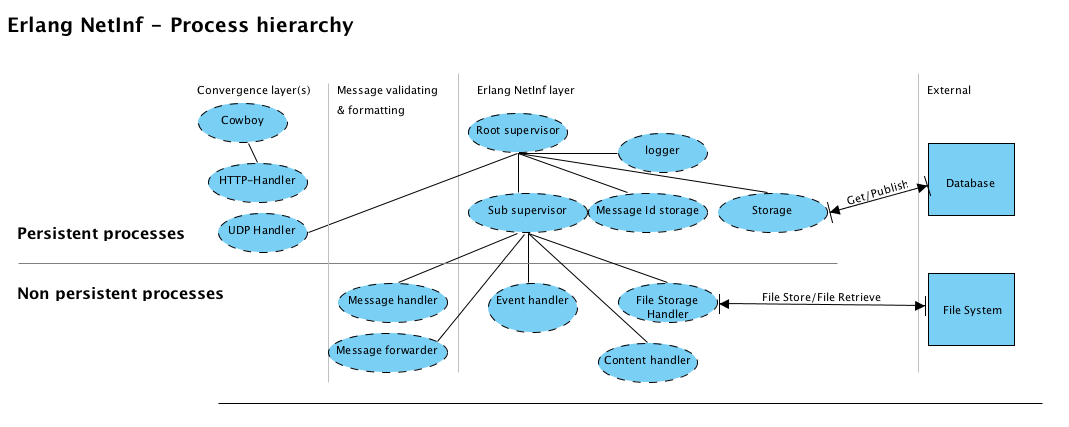
\includegraphics[scale=0.6]{./img/process_hierarchy.png}
\caption{Current system design}
\end{figure}

\subsection{Architecture layers}

The system architecture is divided into four distinct layers a network layer (http, udp) convergence layer, an internal Erlang NetInf layer and a storage layer. Within these layers lie the modules(Erlang processes) which are responsible for specific functions such as sending/receiving convergence layer messages, sanitizing messages, forwarding, accessing databases/file systems and logging.

\subsection{NetInf Messaging}

According to the draft specification(see appendix D-draft) NetInf has three well defined messages which comprise of the core functionality of the system. The following sections describe the purpose and flow of each of these messages.

\subsubsection{Named Data Objects}
In addition to the messaging component, NetInf describes any piece of information as a Named Data Object(NDO). In the current state of networks, the same piece of information is considered to be location based and mutable with many copies of the same information lying around. The purpose of an NDO is to provide a convenient way for the protocol to be able to catalogue and preform operations such as storing, retrieving and finally searching for information and eliminating need for location based information.


\subsubsection{Publish}

NetInf describes a Publish message which consists of the following fields:

\begin{description}
\item[URI]  - Contains the hash of the NDO. It is unique to the peice of information that is going to be published into the system. It is also mandatory.
\item[msgid] - A mandatory field as well and it is a unique number(integer). 
\item[loc1] - An optional field, this is the I.P address of the device that created the information that will be shared.
\item[loc2] - Same as the above.
\item[ext] - An extension field, it is responsible for containing the meta data in JSON format.
\item[rform] - 
\item[fullPut]
\end{description}

\subsubsection{Get}

NetInf describes a Get message which consists of the following fields:

\begin{description}
\item[URI]
\item[msgid]
\item[loc1]
\item[loc2]
\item[ext]
\end{description}


\subsubsection{Search}

NetInf describes a Search message which consists of the following fields:

\begin{description}
\item[msgid]
\item[tokens]
\item[rform]
\item[ext]
\end{description}

